\chapter{Arquitectura}
\label{chap:arquitectura}

\drop{E}{}ste capítulo analiza en detalle, mediante un enfoque top-down, la arquitectura diseñada para dar soporte al sistema propuesto en este proyecto. Se discutirá la funcionalidad de cada módulo perteneciente a la arquitectura, se explicará como están conectados y como fluye la información entre ellos hasta obtener el resultado final. 

\section{Visión general de la arquitectura}
\label{sec:visiongeneral}

La arquitectura diseñada (ver Figura~\ref{fig:arquitectura}) es una arquitectura basada en módulos que contribuye a simplificar significativamente el desarrollo del sistema.

\begin{figure}[!h]
\begin{center}
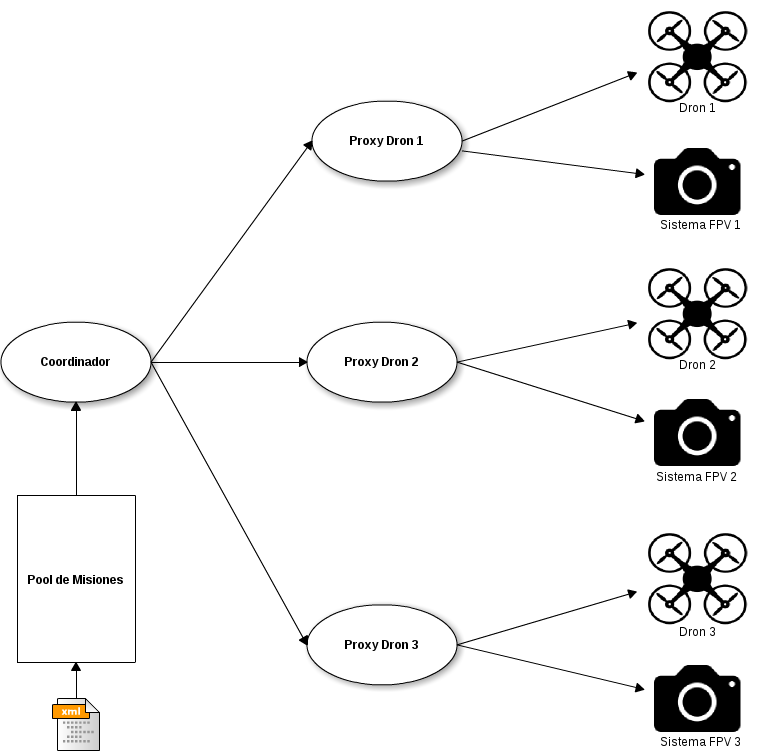
\includegraphics[width=0.63\textwidth]{/arquitectura.png}
\caption[Arquitectura del sistema]{Arquitectura del sistema}
\label{fig:arquitectura}
\end{center}
\end{figure}

Cada módulo representa una clase en la que se definen las propiedades y el comportamiento mediante atributos y funciones. Estas clases son instaciadas en objetos, que se corresponden tanto con objetos reales como con objetos internos del sistema, en los que se realiza la lectura de estas definiciones.

Como se observa, la arquitectura se descompone en cuatro elementos que de forma resumida realizan lo siguiente:
\begin{itemize}
\item \textbf{Coordinador}: realiza una lectura del \textit{Pool de misiones} ordenándolo por prioridad, se encarga de crear instancias del objeto \textit{ProxyDrone}, asignar «waypoints» a vehículos desocupados y ordenar el aterrizaje cuando el \textit{Pool de misiones} este vacío.
\item \textbf{Proxy Dron}: es el responsable a la hora de realizar las operaciones que conciernen al vehículo, como el despegue o la subida de misiones, y de gestionar la conexión con los dispositivos finales, como el \textit{dron} o el \textit{sistema \acs{FPV}}.
\item \textbf{Dron}: Crea una simulación de un vehículo aéreo no tripulado en una localización determinada.
\item \textbf{Sistema FPV}: Captura imágenes en vivo, las analiza y muestra en pantalla los resultados.
\end{itemize} 

En el sistema la información fluye a través de los módulos (ver Figura 3.2), transformándose hasta alcanzar el resultado final. Esto es, los vehículos aéreos se desplazan de manera coordinada a diversas localizaciones y a su vez retransmiten imágenes, que son analizadas para contribuir a mejorar los tiempos de respuesta en situaciones de emergencia.

\begin{figure}[!h]
\begin{center}
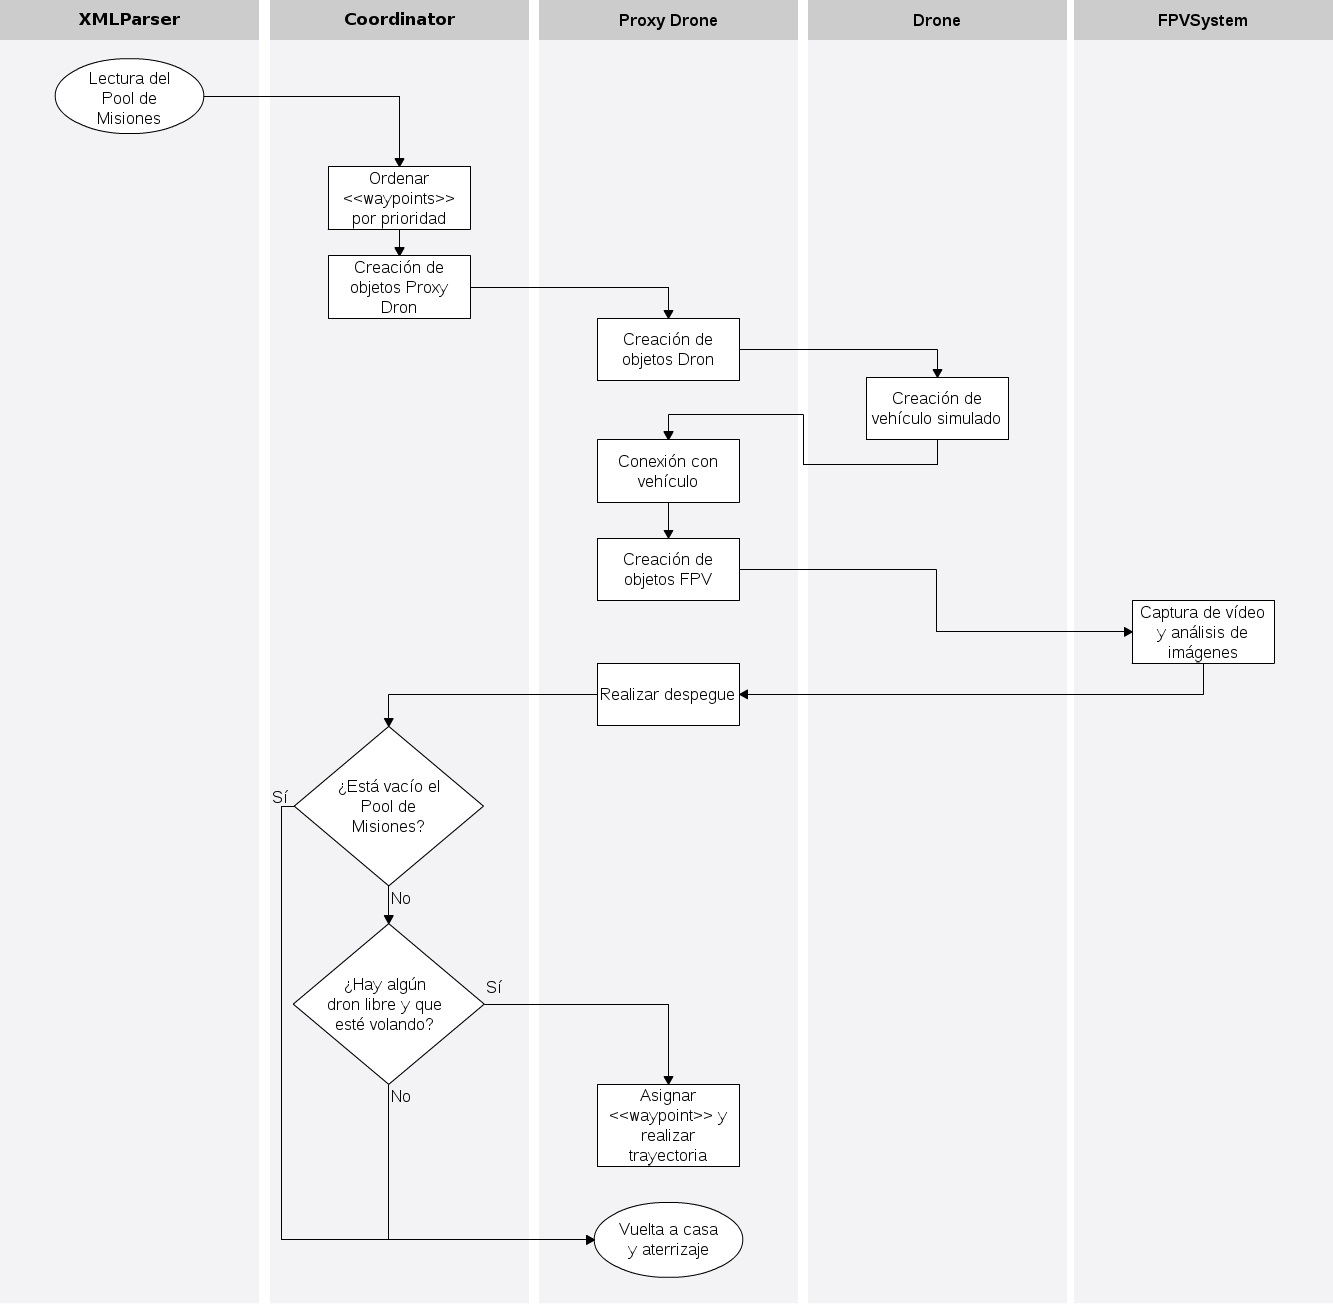
\includegraphics[width=0.8\textwidth]{/Flowchart.png}
\caption[Diagrama de flujo del sistema]{Diagrama de flujo del sistema}
\label{fig:diagflujo}
\end{center}
\end{figure}

\subsection{Coordinador}
\label{sec:coordinador}

\subsection{Proxy Dron}
\label{sec:proxydron}

\subsection{Dron}
\label{sec:dron}

\subsection{Sistema FPV}
\label{sec:sistemafpv}

% Local Variables:
%  coding: utf-8
%  mode: latex
%  mode: flyspell
%  ispell-local-dictionary: "castellano8"
% End:
